\documentclass[dvips,10pt]{book}
%\documentclass[dvips,10pt]{report}

\usepackage{latexsym}
%\usepackage{amstex}
%\usepackage{amssymb}
%\usepackage{amsfonts}
\usepackage{amstext}
\usepackage{amsbsy}
\usepackage{amscd}
\usepackage{makeidx}
\usepackage{graphicx}
%\usepackage{calc}
\usepackage{longtable}

% -- to reduce the margin pages --
\topmargin 2pt
\headsep 20pt
\headheight 2pt

%\textwidth 440pt
%\textheight 690pt
%\oddsidemargin 0pt
%\evensidemargin 0pt

% 19/01/06: EV
\textwidth 490pt
\textheight 700pt
\oddsidemargin -20pt
\evensidemargin -20pt

% --------------------------------

\makeindex

\newcommand{\eyedb}{\textsc{EyeDB} }
\newcommand{\eyedbX}{\textsc{EyeDB}}
\newcommand{\sysra}{SYSRA}
\newcommand{\indexentry}[2]{\item #1 #2}
\newcommand{\chap}[1]{\chapter{#1} \index{#1}}
\newcommand{\sect}[1]{\section{#1} \index{#1}}
\newcommand{\subsect}[1]{\subsection{#1} \index{#1}}
\newcommand{\subsubsect}[1]{\subsubsection{#1} \index{#1}}
%% WARNING \Box does not work with latex2html
%%\newcommand{\iii}{\item[{$\Box$}]}
\newcommand{\rrr}{\item[{$\Box$}]}
\newcommand{\iii}{\item}
\newcommand{\jjj}{\item[-]}
\newcommand{\bi}{\begin{itemize}}
\newcommand{\ei}{\end{itemize}}
\newcommand{\be}{\begin{enumerate}}
\newcommand{\ee}{\end{enumerate}}
\newcommand{\kkk}{\item[ ]}
\newcommand{\sh}[1]{\bf #1}
\newcommand{\ttt}{$\tilde{ }$}
\newcommand{\ttv}[1]{\texttt{#1}}
\newcommand{\ttu}[1]{{\verbsize\texttt{#1}}}
\newcommand{\verbsizex}{\small}
\newcommand{\verbsizey}{\fontsize{8}{\baselineskip}\selectfont}
\newcommand{\verbsize}{\normalsize}
\newcommand{\bugreport}{bug-report@eyedb.org }
\newcommand{\idt}{\mbox{ } - }
\newcommand{\ident}{{\bf \texttt{<}identifier\texttt{>}}}
\newcommand{\grindent}{xxxxxxxxxxxxxxx \= : \kill}
\newcommand{\arr}{\texttt{-$>$}}
\newcommand{\ul}[1]{\underline{#1}}
\newcommand{\uul}[1]{\textit{\texttt{#1}}}
\newcommand{\ixx}{\makebox[3mm]{ }}
\newcommand{\ixy}{\makebox[10mm]{ }}
\newcommand{\ixz}{\\\ixy {- }}

\renewcommand{\normalsize}{\fontsize{9}{11pt}\selectfont}

%\renewcommand{\normalsize}{\fontsize{8}{10pt}\selectfont}

%% The following commands comes from corbaref.tex

\newcommand{\bt}{\begin{tabular}{|p{7cm}|p{7cm}|}}
\newcommand{\et}{\hline \end{tabular} \\ {\vspace{0.6cm}} \\ }

\newcommand{\mt}[1]{\hline \multicolumn{2}{|c|}{\centerline{{\bf interface #1}
   \emph{mapped from} {\bf class #1}}}}

\newcommand{\Desc}[1]{\hline \multicolumn{2}{|l|}{\emph{#1}}}

\newcommand{\mTT}[2]{\hline \multicolumn{2}{|c|}
   {\centerline{{\bf interface #1} \emph{extends} {\bf #2}
   \emph{mapped from} {\bf #1}}}}


\newcommand{\mT}[2]{\hline \multicolumn{2}{|c|}{\centerline{{\bf #1}
\emph{mapped from} {\bf #1}}}}

\newcommand{\att}{\hline \hline {\bf Attribute} & {\bf Description}}
\newcommand{\mtt}{\hline \hline {\bf Method} & {\bf Description}}
\newcommand{\mf}{\emph{mapped from }}

\newcommand{\satt}[1]{\hline \multicolumn{2}{|c|}
   {\centerline{\emph{attributes inherited from} {\bf #1}}}}

\newcommand{\smtt}[1]{\hline \multicolumn{2}{|c|}{
   \centerline{\emph{methods inherited from} {\bf #1}}}}

\newcommand{\sets}[1]{sets the #1 \emph{value} in the Object \emph{o} at the \emph{ind}}

\newcommand{\Gets}[1]{gets the #1 value in the Object \emph{o} at the \emph{ind}}

%\setcounter{secnumdepth}{-1}
%\addtocounter{secnumdepth}{2}

\renewcommand{\thesection}{\arabic{section}}
\renewcommand{\thesubsection}{\arabic{section}.\arabic{subsection}}
\renewcommand{\thechapter}{}

\begin{document}
\normalsize


\input{version}
\newcommand{\mantitle}{\textsc{Overview} }

\thispagestyle{empty}

\mbox{ }
\\
\vspace{3 cm}
\\
%{\bf{\Huge E{\LARGE YE}DB} \hspace{0.cm} {\LARGE Programming Manual}}
{\bf{\Huge E{\LARGE YE}DB} \hspace{0.cm} {\Huge \mantitle}}
\\
%\newcommand{\rulewidth}{12.2cm}
\newcommand{\rulewidth}{15.4cm}
\rule{\rulewidth}{1.6mm}
\begin{flushright}
{\large Version \eyedbversion}
\end{flushright}
\mbox{ }
\\
\vspace{11 cm}
\\
\begin{flushright}
{\large January 2006}
\end{flushright}

\newpage

\thispagestyle{empty}

\mbox{ }
\\
\vspace{1cm}
\\
Copyright {\copyright} 2001-2006 SYSRA
\\
\vspace{1cm}
\\
Published by \sysra
\\
30, avenue G\'en\'eral Leclerc
\\
91330 Yerres - France
\\
\\
home page: http://www.eyedb.org
\\
\\
bug report: \bugreport


\tableofcontents

\newcommand{\bigcaps}[1]{\uppercase{#1}}

\hyphenation{cor-ba}
\hyphenation{data-bases}
\hyphenation{HuGe-Map}

%\newcommand{\ixx}{\makebox[3mm]{ }}
%\newcommand{\ixy}{\makebox[10mm]{ }}
%\newcommand{\ixz}{\\\ixy {- }}
\newcommand{\bii}{\\}
\newcommand{\eii}{\\\\}
\newcommand{\oidx}{\emph{oid}}
\newcommand{\oid}{{\oidx} }
\newcommand{\class}[1]{class \texttt{#1}}
\newcommand{\instance}[1]{instance of the \class{#1}}
\newcommand{\instances}[1]{instances of the \class{#1}}

\chapter*{Overview}

This document presents a quick overview of \eyedbX. All the topics introduced
here are developped in the other documents.

%------------------------------------------------------------------------- 
\section{Introduction}

The key features of the \eyedb OODBMS are:
\bi
\item {\bf standard OODBMS features}:
persistent typed data management;
client/server model; transactional services; recovery system;
expressive object model; inheritance; integrity constraints; methods;
triggers; query language; application programming interfaces~\ldots
\item {\bf language orientation}:
a definition language based on the ODMG Object Definition
Language (ODL);
a query language based on the ODMG Object Query Language (OQL);
several manipulation language bindings (at least C++ and Java),
\item {\bf genericity and orthogonality of the object model}:
inspired by the SmallTalk, LOOPS, Java and ObjVlisp object models
(i.e. every class derives from the \class{object} and can
be manipulated as an object);
type polymorphism;
binary relationships;
literal and object types;
transient and persistent objects;
method and trigger overloading;
template-based collections such as set, bag and array;
multi-dimensional and variable size dimensional arrays,
\item {\bf support for large databases}: 
databases up to several Tb (tera-bytes),
\item {\bf efficiency}:
database objects must be directly mapped within
the virtual memory space; object memory copy must be
reduced to the minimum; clever caching policies must be implemented,
\item {\bf scalability}: programs must be able to deal with hundred
of millions of objects without loss of performance.
\ei
We describe below how \eyedb meets these requirements.
Section 2 introduces the storage manager subsystem.
In section 3, the object model is exposed.
Sections 4 and 5 describe the \eyedb object definition language and
query language.
Sections 6 and 7  deal with the C++ and Java bindings.

%------------------------------------------------------------------------- 
\section{The Architecture}
\eyedb is based on a client/server architecture as shown in Figure
\ref{arch}.
\\
\\
The \eyedb server is composed of:
\bi
\item the server protocol layer based on Remote Procedure Call (RPC),
\item the object model implementation,
\item the OQL engine,
\item the storage manager subsystem.
\ei
A client is composed of:
\bi
\item the user application code,
\item the C++ (resp. Java) API implementing the C++ (resp. Java) binding,
\item the client protocol layer based on RPC.
\ei
\begin{figure*}[!th]
\centering
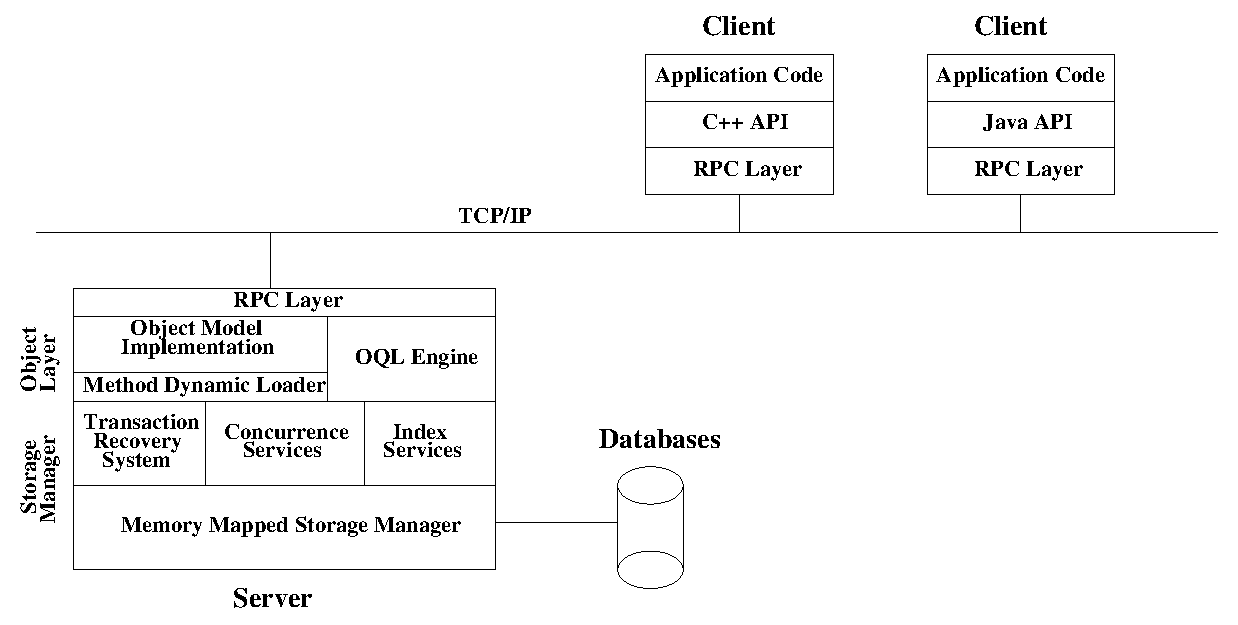
\includegraphics[height=60mm]{figures/arch.eps}
\caption{The \eyedb Architecture}
\label{arch}
\end{figure*}
%------------------------------------------------------------------------- 
\section{The Storage Manager Subsystem}
\eyedb is based on a client/server architecture.
The server kernel is the storage manager subsystem providing the
\vspace{2mm}
following main services:\\
\ixy - persistent raw data management,\\
\ixy - transactional services,\\
\ixy - recovery system,\\
\ixy - B-tree and hash indexes,\\
\ixy - multi-volume database management.\\ \\
The storage manager can be used independently from \eyedbX.

%------------------------------------------------------------------------- 
\subsection{Raw Data Management}
The central concept of the storage manager is the raw object.
A raw object is a piece of persistent raw data tied to an object identifier
named \oid.
\\
An \oid identifies a raw object in a unique way within a set of databases.
It is
generated by the storage manager at raw object creation.
\\
An \oid is composed of three fields: the storage index, the database identifier
and a random generated magic number.
\\
The first field identifies the object physical location
within a database volume.
The second one identifies a database and the last one ensures more
security in the object identification process.
\\
\\
The storage manager is responsible for the management of raw objects:
\bi
\item raw object creation (\emph{storage allocation, oid allocation,
 object storage}),
\item raw object update (\emph{contents modification}),
\item raw object reading,
\item raw object deleting (\emph{oid deallocation,  storage deallocation}),
\item raw object resizing (\emph{storage reallocation, 
object moving}),
\item raw object locking and unlocking (\emph{share locking, exclusive locking, private locking}),
\item raw object access control
\ei

%------------------------------------------------------------------------- 
\subsection{Memory Mapped Architecture}
The storage manager is based on a memory mapped architecture. Database
volumes are mapped within the server virtual memory space.
\\
Due to some 32-bit system limitations, the databases greater than 2Gb cannot
be mapped as a whole.
\\
\\
The storage manager implements a segment-based mapping algorithm:
when reading an object, the storage manager checks if the
corresponding storage piece is mapped within its virtual memory space. If it is
not mapped, it maps a large segment of data around the raw object,
eventually extending a neighboring segment.
\\
If the total mapped size is more than the system maximum, it
unmaps the less recent used mapped segment.
On 64-bit system, this algorithm is not needed as databases up to
several Tb (i.e. tera-bytes) can be mapped at whole within the virtual
 memory space.
\\
Currently, the storage manager can deal with databases up to one
Tb.
\subsection{Transactional Services}
  The storage manager provides standard transaction services which
  guarantees atomicity,  consistency, isolation and integrity within
  a database.
\\
  Its transaction unit is based on a two-phase locking protocol.
  The protocol requires that each transaction issues lock and unlock requests
  in two phases:
\bi
\item growing phase: a transaction may obtain locks but may not release
any lock.
\item shrinking phase: a transaction may release locks but may not obtain
any new lock.
\ei
Initially, a transaction is in the growing phase. The transaction acquires
locks as needed. Once the transaction releases a lock, it enters the
shrinking phase and no more lock requests may be issued.
\\
\\
The storage manager provides different transaction locking modes:
read and write shared,
read shared and write exclusive, read and write exclusive or
database exclusive.
\\
It provides immediate deadlock detection.
\subsection{The Recovery System}
The storage manager provides a simple but efficient recovery system against
failures:
\bi
\item client failure: the transaction is automatically aborted by the server.
\item server failure or operating system failure: the current transactions
  will be automatically aborted on the next database opening.
\item the disk failure recovery is not supported: this is a deliberate
choice of simplicity since storage consistency
can rely on the RAID technology or transactional file systems now available
on modern operating systems.
\ei

\subsection{B-Tree and Hash Indexes}
The storage manager provides support for B-Tree and Hash indexes.
\\
The B-Tree index provides fixed size raw data indexation,
efficient exact match query and range query.
\\
The Hash index provides variable size raw data indexation
and efficient exact match query. The hash key function can
be provided by the client.

\subsection{Multi-Volume Database Management}
The database storage unit is the volume files. A database can contains
up to 512 volumes each one up to 2Gb on a 32-bit file system interface,
or up to several tera-bytes on a 64-bit file system interface.
The storage manager provides facilities to add, move, resize and reorganize
database volumes.
\section{The Object Model}
The \eyedb object model is inspired by the SmallTalk, LOOPS, ObjVlisp, Java
and ODMG models.
\\
\\
The main three class abstractions are the \class{object} which is
the root class, the \class{class} and the \class{instance} as shown in
Figure \ref{objmod}.
\\
\\
Generally speaking, the instantiation of a \class{X} gives an \instance{X}.
\begin{figure*}[!th]
\centering
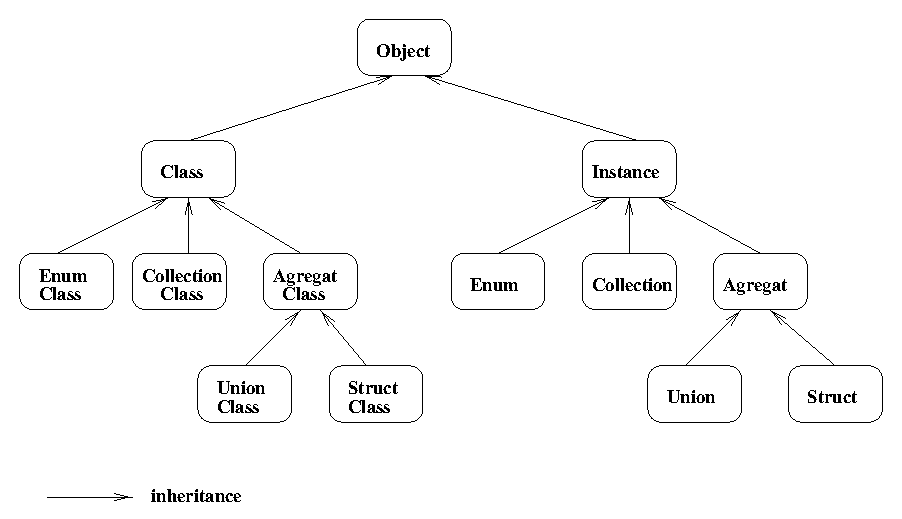
\includegraphics[height=60mm]{figures/objmod.eps}
\caption{Partial Native Object Model}
\label{objmod}
\end{figure*}
\\
An instance cannot be instantiated except the \instances{class} or its
subclasses: the instantiation of an \instance{class} is an \instance{instance}
(i.e. an instance of the \class{instance}).
\\
\\
If \emph{new()} denotes the instantiation method:
\\
\\
\ixx\ttv{struct\_class} \textsf{Person} =\\
\ixy  \ttv{struct\_class}\texttt{->}\emph{new}(name = "Person", ...)
\\
\\
\textsf{Person} is an \instance{struct\_class} that can be instantiated:
\\
\\
\ixx \ttv{struct} \textsf{john} =\\
\ixy  \textsf{Person}\texttt{->}\emph{new}(name = "john", age = 32)
\\
\\
\textsf{john} is an \instance{struct} that cannot be instantiated
\\
\\
\ixx\ttv{struct\_class} \textsf{Employee} =\\
\ixy  \ttv{struct\_class}\texttt{->}\emph{new}(name = "Employee",\\
\ixy   parent = \textsf{Person}, ...)
\\
\\
\ixx \ttv{struct} \textsf{henry} =\\
\ixy  \textsf{Employee}\texttt{->}\emph{new}(name = "henry",\\
\ixy  salary = 10000)
\\
\\
Figure \ref{objmod2} shows this instantiation mechanisms.
\\
\\
Note that as the \class{class} derives from the \class{object},
an \instance{class} can be manipulated like any \instance{object}.
\\
\\
The native \eyedb object model is composed of 76 classes
such as the \class{collection}, the \class{method},
the \class{constraint}, the \class{index}, the \class{image}
and so on.
\\
\eyedb object model supports all standard built-in types:
\ttv{16-bit, 32-bit} and \ttv{64-bit integer, character, string, 64-bit float}.
\\
\\
An instance can be \uul{transient} or \uul{persistent}:
\bi
\item an instance is \uul{transient} if its lifetime does not exceed the
lifetime of the unit of execution in which it is manipulated.
\item otherwise the instance is \uul{persistent}.
\ei
A \uul{persistent} instance can be \uul{object} or \uul{literal}:
\bi
\item an \uul{object} \uul{persistent} instance has an unique identifier
(i.e. an \oidx)
\item a \uul{literal} \uul{persistent} instance has
no identifier.
\ei
\begin{figure*}[!th]
\centering
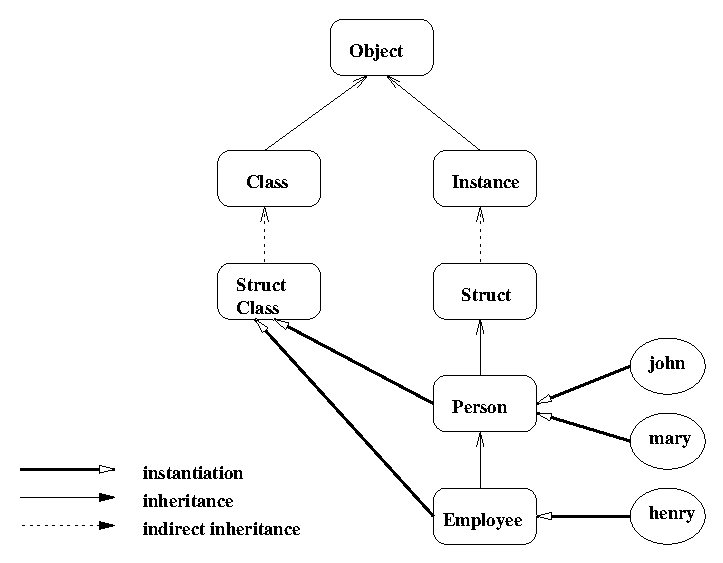
\includegraphics[height=60mm]{figures/objmod2.eps}
\caption{Applicative Object Model Example}
\label{objmod2}
\end{figure*}
\subsection{Class Structure}
A class is composed of a name, a parent class (except for the
\class{object} which is the root class), a set
of attributes, a set of methods and a set of triggers:
\bi
\item an attribute is composed of a type, an optionnal array modifier and
is \uul{literal} or \uul{object}. For instance, using the \eyedb ODL
language:
{\verbsize
\begin{verbatim}
   attribute int32 age
\end{verbatim}
}
is a \uul{literal} attribute of type \ttv{int32} with no array modifier,
while the following attribute:
{\verbsize
\begin{verbatim}
   attribute Person *children[10]
\end{verbatim}
}
is a fixed-size array of \uul{object} of type \ttv{Person}.

\item a method is a unit of execution tied to a class.
\\
A method can be either a class method or an instance method.
\item a trigger is a unit of execution tied to a class.
Triggers are applied to instances of this class on a given event.
\\
For example, a trigger \ttv{update\_before} tied to the \class{X}
means that before the update of any \instance{X}, the trigger will
be called.
\\
A method or a trigger can be overloaded by the sub-classes.
\\
\\
\eyedb supports the following trigger events: \ttv{create\_before},
\ttv{create\_after},
\ttv{update\_before},
\ttv{update\_after},
\ttv{load\_before},
\ttv{load\_after},
\ttv{remove\_before},
\ttv{remove\_after}.
\ei
\subsection{Type Polymorphism}
The two language bindings, C++ and Java, and \eyedb OQL supports
type polymorphism: variables may be bound by instances of different types.
\\
This is a direct consequence owing to the fact that any \eyedb class
inherits from the \class{object},
\\
\\
The possibility of manipulating polymorphic objects is a
major contribution of object orientation.
\subsection{The Collection Type}
A collection is composed of elements of the same type.
\\
The elements can be either \uul{literal} or \uul{object}.
\\
\\
If the collection element type is the \class{object}, then
the collection can contain instances of any class, as all
classes inherit from the \class{object}.
\\
\\
The collection types supported by \eyedb are the \ttv{set}, the
\ttv{bag} and the \ttv{array}:
\bi
\item an \instance{set} is an unordered collection with no duplicates allowed,
\item an \instance{bag} is an unordered collection that may contain duplicates,
\item an \instance{array} instance is dynamically sized ordered collection.
\ei
The collection type is a major concept of the \eyedb object model.

\subsection{Relationships}
The \eyedb object model supports only binary relationships, i.e. relationships
between two types.
\\
A binary relationship may be one-to-one, one-to-many or many-to-many
depending on the cardinality of the related types.
Relationships are not named.
\\
\\
\eyedb maintains the referential integrity of
relationships. This means that if an object that participates
in a relationship is removed, then any traversal path to that object
is also removed.
\\
\eyedb supports object-valued attribute: this kind of attribute enables one
object to reference another without expectation of referencial integrity.
An object-valued attribute implements a unidirectionnal relationship:
in this case, \eyedb does not guarantee the referential integrity.
Note that such a unidirectionnal relationship is not called a relationship.
\\
\\
The example introduced in the section \emph{The Object Definition Language}
illustrates the use of relationships and object-valued attributes.
\subsection{Constraints}
\eyedb supports all standard constraints:
\bi
\item the \ttv{not null} constraint on a attribute within
a \class{X} means that no \instances{X} can have
this attribute value not assigned.
\item the \ttv{unique} constraint on a attribute within a \class{X}
means that one cannot create an \instance{X} which has the same 

attribute value than an existing instance in the database.
\item the \ttv{cardinality} constraint on an \instance{collection} means
that the count of this collection must follow this cardinality constraint.
\ei
\section{The Object Definition Language}
The \eyedb Object Definition Language (ODL) is a language
based on the ODMG ODL to define the specifications of object types.
\\
ODL is not intended to be a full programming language, it is a definition
language for objet specifications.
\\
\\
Like ODMG ODL, \eyedb ODL defines classes (inheritance and
attributes), relationships and method signatures.
\eyedb ODL extends the ODMG ODL to allow the definition of
attribute constraints (notnull, unique, collection cardinality), index
specifications and trigger declarations. Unlike ODMG ODL, any instance
of a class can be used either as a \uul{literal} or as
an \uul{object}. \eyedb ODL also allows the user to specify whether a method
is backend (i.e. server side) or frontend (i.e. client side),
and whether it is a class or instance method.
\\
\\
Here is a simple example of an \eyedb ODL construct:
{\verbsize
\begin{verbatim}
enum CivilState {
  Lady = 0x10,
  Sir  = 0x20,
  Miss = 0x40
};

class Address {
  attribute string street;
  attribute string<32> town;
};

class Person {
  attribute string name;
  attribute int age;
  attribute Address addr;
  attribute CivilState cstate;
  attribute Person * spouse inverse Person::spouse;
  attribute set<Car *> * cars inverse Car::owner;
  attribute Person *children[];

  instmethod void change_address(in string street,
                                 in string town,
                                 out string oldstreet,
                                 out string oldtown);

  classmethod int getPersonCount();
  index on name;
};

class Car {
  attribute string brand;
  attribute int num;
  attribute Person *owner inverse Person::cars;
};

class Employee extends Person {
  attribute long salary;
  Person *boss;
};
\end{verbatim}
}
This example illustrates all the concepts that we described
previously.
\\
The \class{Person} is composed of a number of attributes
each of one having an interesting particularity.
\\
The \ttv{name} attribute is a variable size character array, i.e. a string.
\\
This attribute is \uul{literal}, which means that it has no identifier within
a database. The hint \ttv{index} means that this attribute should be
indexed to provide efficient query according to the attribute value.
\\
\\
The \ttv{age} attribute is a simple \uul{literal} \ttv{32-bit integer}.
\\
\\
The \ttv{addr} attribute is a \uul{literal} user type attribute.
As this attribute is \uul{literal}, the type attribute, \ttv{Address},
must have been defined before, which is the case.
\\
\\
The next attribute \ttv{spouse} has two interesting particularities:
\be
\item a \emph{*} character follows the user type \emph{Person}, meaning that this
attribute is not a \uul{literal} but an \uul{object} (i.e. with
an identifier). The \emph{*} character
means a reference to an object.
\item the hint \ttv{(invers Person::spouse} following \ttv{spouse}
means that this attribute is a relationship.
\\
As the attribute \ttv{spouse} is not a collection and the target attribute
\ttv{spouse} is not a collection, this is a one-to-one relationship.
\ee
The \ttv{cars} attribute has also several interesting particularities:
\be
\item as a \emph{*} character follows the user type, this is an \uul{object}.
\item this attribute is a \ttv{set} whose elements are \uul{object}
of type \ttv{Car}.
Note that the user type \ttv{Car} is defined after.
\item the hint \ttv{(inverse Car::owner} following \ttv{cars}
means that this attribute is a relationship whose target is the
\ttv{owner} attribute within the class \ttv{Car}.
\\
As the source attribute \ttv{cars} is a collection and the target
attribute \ttv{owner} is not a collection, the relationship is 
a many-to-one relationship.
\ee
As indicated by the keyword \ttv{instmethod}, the method        
\ttv{change\_address} is an instance method. Note that this keyword
is optionnal as this is the default.
\\
The method \ttv{getPersonCount} is a class method as indicated by
the \ttv{classmethod} keyword.
\\
\\
The class \ttv{Employee} inherits from the class \ttv{Person}
as indicated by the keyword \ttv{extends}.
It introduces two attributes \ttv{salary}, a \uul{literal} integer
attribute and \ttv{boss}, an \uul{object} attribute which reference
an \instance{Person}. Note that as there is no relationship
indication (i.e. \ttv{inverse} keyword), the \ttv{boss} attribute is an
object-valued attribute (i.e. a unidirectionnal relationship):
in this case, \eyedb does not guarantee the referential integrity.
\section{The Object Query Language}
\eyedb provides a query language based on the ODMG OQL.
\\
Although \eyedb OQL is not an OML (i.e. an Object Manipulation Language),
most of the common language operations can be performed (arithmetic
and logical operations, string manipulation, flow control,
function definition) as well as query constructs.
\\
\\
\eyedb OQL adds a few features from the ODMG OQL such as flow control
(\ttv{if else}, \ttv{for}, \ttv{while}), function definition,
an assignement operator, and regular expression operators.
\\
\\
For instance the following examples are \eyedb OQL legal constructs:
{\verbsize
\begin{verbatim}
function max(x, y) {return (x > y ? x : y);};

function fib(n) {
  if (n < 2)
    return n;
  return fib(n-1) + fib(n-2);
};

for (x in list(1, 2, 3, 4))
  fib(x);

for (x := 0; x < 10; x++)
  fib(x);
\end{verbatim}
}
Note that the previous code does not perform any query.
\\
\\
The following code perform queries:
{\verbsize
\begin{verbatim}
select Person;          // returns the OIDs of all Person instances

select x from Person;   // idem

select Person.name =  "john"; // returns the Person whose name is "john"

select Person.name ~ "^a.*b"; // returns the instances whose name matches
                              // the regular expression

select Person.name !~~ "ja" // returns the Person whose name does
                            // not matches the regular expression in a case
                            // insensitive way.

select x from Person x where x.age > 2 && // returns Person  whose age is between
                       x.age < 10;        // 2 and 10.

select Person.name;     // returns all Person names

select x.name from Person x;  // idem

for (x in (select Person)) // for each Person
 if (x.name ~ "^j")        // whose name matches
   x.name := \"_\" +       // the regular expression
       x.name;;            // "j", adds a "_" before
                           // the name.

// set the age of the Person whose name
// is "john" to 20:
(select Person.name = "john").age := 20;
\end{verbatim}
}
\section{The C++ Binding}
The C++ binding maps the \eyedb object model into C++ by introducing
a generic API and a tool to generate a specific C++ API from
a given schema, built upon the generic API.
\\
\\
Each class in the \eyedb object model is implemented as a C++
class within the C++ API: there is a one-to-one mapping between
the object model and the C++ API.

\subsection{Transient and Persistent Objects}
There are two types of runtime objects: persistent runtime objects and
transient runtime objects.
\\
A runtime object is persistent if it is tied to a database object.
Otherwise, it is  transient.
\\
\\
By default, \eyedb does not
provide an automatic synchronisation between persistent runtime objects
and database objects.
\\
When setting values on a persistent runtime object, we do not modify
the tied database object.
One must call the \ttv{store} method on the persistent runtime object
to update the tied database object.
\\
\\
Note that any persistent runtime object manipulation must be done
in the scope of a transaction.
\\
\\
To illustrate object manipulations, we introduce a simple concrete
example using the schema-oriented C++ API, based on the previous ODL
example construct:
{\verbsize
\begin{verbatim}
 // connecting to the EyeDB server
 eyedb::Connection conn;
 conn.open();

 // opening database dbname
 personDatabase db(dbname);
 db.open(&conn, eyedb::Database::DBRW);

 // beginning a transaction
 db.transactionBegin();

 // creating a Person
 Person *p = new Person(&db);

 // setting attribute values
 p->setCstate(Sir);
 p->setName(name);
 p->setAge(age);

 p->getAddr()->setStreet("voltaire");
 p->getAddr()->setTown("paris");

 // creating two cars
 Car *car1 = new Car(&db);
 car1->setBrand("renault");
 car1->setNum(18374);

 Car *car2 = new Car(&db);
 car2->setBrand("ford");
 car2->setNum(233491);

 // adding the cars to the created person
 p->addToCarsColl(car1);
 p->addToCarsColl(car2);

 // storing all in database
 p->store(eyedb::RecMode::FullRecurs);

 // committing the transaction
 db.transactionCommit();
\end{verbatim}
}
A few remarks about this code:
\be
\item the statement \ttv{Person *p = new Person(\&db)} creates a
transient runtime object. This runtime object is not tied to any
database object until the \ttv{store} method has been called.
\item all the selector and modifier methods such as \ttv{setName},
\ttv{getAddr}, \ttv{addToCarsColl} have been generated by the \eyedb
ODL compiler from the previous ODL construct.
\item the \ttv{eyedb::RecMode::FullRecurs} argument to the \ttv{store}
method allows the user for storing each object related the calling instance:
so the runtime object \ttv{car1} and \ttv{car2} within the \ttv{cars}
collection will be automatically stored using the \ttv{store} method
with this argument.
\item the call to \ttv{transactionCommit} ensures that the database changes
will be kept in the database.
\ee
\section{The Java Binding}
The use of the Java language for an \eyedb binding has been motivated by
several reasons:
\be
\item Java is architecture independent,
\item Java is valuable for distributed network environment,
\item Java has a very rich builtin library,
\item Java is secure,
\item Java is easier to program than C++.
\ee
The Java binding is very close from the C++ binding: the
class interfaces are identical, the functionalities
are the same; only the language is slightly different.
\\
\\
The previous C++ code is here translated for the \eyedb Java API:
{\verbsize
\begin{verbatim}
 // connecting to the EyeDB server
 org.eyedb.Connection conn = new org.eyedb.Connection();

 // opening database dbname
 person.Database db = new person.Database(dbname);
 db.open(conn, org.eyedb.Database.DBRW);

 // beginning a transaction
 db.transactionBegin();

 // creating a Person
 Person p = new Person(db);

 // setting attribute values
 p.setCstate(CivilState.Sir);
 p.setName(name);
 p.setAge(age);

 p.getAddr().setStreet("voltaire");
 p.getAddr().setTown("paris");

 // creating two cars
 Car car1 = new Car(db);
 car1.setBrand("renault");
 car1.setNum(18374);

 Car car2 = new Car(db);
 car2.setBrand("ford");
 car2.setNum(233491);

 // adding the cars to the created person
 p.addToCarsColl(car1);
 p.addToCarsColl(car2);

 // storing all in database
 p.store(org.eyedb.RecMode::FullRecurs);

 // committing the transaction
 db.transactionCommit();
\end{verbatim}
}
As shown in this example, the code is absolutely identical except
that that some \ttv{->} in C++ are replaced by a \ttv{.} character
in Java.
\\
The only difference that does not appear in our examples is the
object memory management. In the C++ example, one should release
all the allocated objects; it is not necessary in Java.
\section{Conclusion}
This chapter provided a quick overview of the \eyedb OODBMS. The next
chapter provides a more pragmatical approach of \eyedb by working through 
a simple
example of defining an ODL schema and manipulating persistent data in OQL,
C++ and Java.

\end{document}
